\documentclass[USenglish,oneside,twocolumn]{article}

\usepackage[utf8]{inputenc}%(only for the pdftex engine)
%\RequirePackage[no-math]{fontspec}%(only for the luatex or the xetex engine)
\usepackage[big]{dgruyter_NEW}
% allow URL breaks on dashes
\def\UrlBreaks{\do\/\do-}

% math environment
\usepackage{mathtools}
\usepackage{amsmath}
\usepackage{amssymb}
\usepackage[%
    lambda, advantage, operators, sets, adversary, landau, probability, notions,
    logic, ff, mm, primitives, events, complexity, asymptotics, keys,
]{cryptocode}

% prettier line breaks
\usepackage{microtype}

% figures
\usepackage{graphicx}
\usepackage[position=bottom]{subfig}
\usepackage{tikz}
\usepackage{tikz-qtree}
\usetikzlibrary{shapes.misc,positioning,arrows,snakes,calc}

% colors
\usepackage{color}
\usepackage{colortbl}
\definecolor{rgddTeal}{HTML}{009999}
\definecolor{rgddLime}{HTML}{809933}
\definecolor{rgddPurple}{HTML}{993380}
\definecolor{rgddDred}{HTML}{E04644}
\definecolor{rgddDgreen}{HTML}{008000}
\definecolor{rgddDblue}{HTML}{2809B2}

% custom commands
\newcommand{\TODO}[1]{\textcolor{red}{TODO:} \emph{#1}}

 
\DOI{foobar}

\cclogo{
\includegraphics{by-nc-nd.pdf}}
  
\begin{document}
  %\author*[1]{Corresponding Author}
  %\author[2]{Second Author}
  %\author[3]{Third Author}
  %\author[4]{Fourth Author}
  %\author[5]{Fifth Author}
  %\affil[1]{Affil, E-mail: email@email.edu}
  %\affil[2]{Affil, E-mail: email@email.edu}
  %\affil[3]{Affil, E-mail: email@email.edu}
  %\affil[4]{Affil, E-mail: email@email.edu}
  %\affil[5]{Affil, E-mail: email@email.edu}

  \title{\huge%
	Incremental and Privacy-Preserving Certificate Transparency Support Within
	the Tor Network
  }
  \runningtitle{%
	Incremental and Privacy-Preserving Certificate Transparency Support Within
	the Tor Network
  }
  %\subtitle{...}

  \begin{abstract}
      {The security of the web has greatly improved in the last couple of years. HTTPS
is now the default, with browsers moving towards warning when unencrypted
connections are made. The Certificate Authority (CA) system has also improved.
The advent of mandatory Certificate Transparency (CT) logging of all
certificates issued by CAs---enforced by web browsers---has made the
weakest-link setting of the CA system more sustainable. However, Tor and its Tor
Browser, based on Firefox, is missing support for CT.

In this paper, we present designs for privacy preserving and
incrementally-deployable support for CT in Tor. Our designs go beyond
the support for CT found in browsers like Google Chrome or Apple's
Safari: we aim to do more than detect CA misbehavior supporting
man-in-the-middle or impersonated HTTPS connections from Tor Browser.
We also create independent public evidence of CT log misbehavior in
support of this. Our base design shares observed certificates in Tor
Browser with other CT logs. Associated privacy leaks of browsing
behavior of Tor users are minimized through the use of indirect
routing and randomized delay of certificate reporting through relays
in the Tor network.

We also present two possible extensions to our base design that can also detect
CT log misbehavior. One extension makes a slight change to the API and operation
of CT logs, the other adds more complexity to Tor but in turn completely removes
all trust placed in CT log operators. Detecting CT log misbehavior is
particularly important for the wider web, since CT as currently deployed lacks
strong mechanisms necessary for reducing trust in CT log operators.
We turn Tor into a system for maintaining a probabilistically-verified view of
the CT log ecosystem as available from Tor’s consensus.
}
  \end{abstract}

  \keywords{Certificate Transparency, Tor}
  %\classification[PACS]{}
  %\communicated{...}
  %\dedication{...}

  \journalname{Proceedings on Privacy Enhancing Technologies}
  \DOI{Editor to enter DOI}
  \startpage{1}
  \received{..}
  \revised{..}
  \accepted{..}

  \journalyear{..}
  \journalvolume{..}
  \journalissue{..}
 
  \maketitle
  \section{Introduction} \label{sec:introduction}
Metrics reported by Google and Mozilla reveal that encryption on the web
skyrocketed the past couple of years: at least 85\% of all web pages load using
Transport Layer Security (TLS) as part of
HTTPS~\cite{google-metrics,mozilla-metrics}. An HTTPS connection is initiated by
a TLS handshake where the client web browser requires that the web server
presents a valid certificate to authenticate the identity of the server (e.g.,
to make sure that the client who wants to visit \url{mozilla.org} really is
connecting to Mozilla, and not, say, Google). A certificate is considered valid
if it is digitally signed by a Certificate Authority (CA) that the browser
trusts. Each CA is trusted to certify (sign) that specific cryptographic
key-material as part of a certificate belongs to a particular domain name.

The CA trust model suffers from \emph{weakest-link} security: web browsers trust
hundreds of CAs, and it is enough to compromise a single CA to get a certificate
mis-issued in the name of a target domain~\cite{ca-ecosystem,https-sok}.
Motivated by this issue manifested by prominent CA compromises---such as the
issuance of a fraudulent certificate for \url{google.com} by DigiNotar in
2011\footnote{\url{https://web.archive.org/web/20200521135444/https://arstechnica.com/information-technology/2011/08/earlier-this-year-an-iranian/}}---several
major browser vendors have mandated that certificates issued by CAs must be
included into trusted Certificate Transparency (CT) logs for browsers to trust
them~\cite{ct/a,ct,ct/bis}. The idea behind CT is that, by making all issued
certificates transparent, mis-issued certificates can be detected \emph{after}
issuance and appropriate actions taken to keep the wider web safe (e.g.,
revocation of certificates, suspected compromises investigated, or trust in
misbehaving CAs removed from browsers). Browsers that wish to benefit from CT
augment the validation done by the browser during the TLS handshake to also
require cryptographic proof from the server that the presented certificate has
been included into CT logs trusted by the browser. Notable browsers with
mandatory CT support by default are Google Chrome and Apple's Safari
\cite{chrome-policy,safari-policy}. Unfortunately, Mozilla's Firefox lacks
support but has a partial implementation.

Beyond security on the web, anonymous access to the web has also matured. In
particular, Tor with its Tor Browser (TB) today have millions of daily users
\cite{tor,mani}, and effort is ongoing into maturing the technology for wider
use\footnote{\url{https://web.archive.org/web/20200528174708/https://mozilla-research.forms.fm/mozilla-research-grants-2019h1/forms/6510}}.
The basis of TB is Firefox, where TB then enables anyone to browse the web
anonymously by relaying traffic between browser and web server through the Tor
network, consisting of thousands of voluntary-run relays across the globe. 

Just like attackers may be interested in breaking HTTPS, attackers are
interested in breaking the anonymity provided by Tor with the goal of
deanonymizing users. One common deanonymization technique, known to be used in
practice by, e.g., law enforcement, is to compromise TB instead of directly
circumventing the anonymity provided by the Tor
network\footnote{\url{https://web.archive.org/web/20200528175225/https://zerodium.com/tor.html}}.
Modern web browsers like TB (Firefox) are one of the most complex types of
software in wide use today. This complexity and wide use leads to security
vulnerabilities and incentives for exploitation. For example, the exploit
acquisition platform Zerodium offers up to \$100,000 for a zero-day exploit
against Firefox that leads to remote code execution and local privilege
escalation\footnote{\url{https://web.archive.org/web/20200521151311/https://zerodium.com/program.html}}
(i.e., full control of the browser for the attacker).

An attacker that wishes to use such an exploit to compromise and then ultimately
deanonymize a TB user has to deliver the exploit to TB\@. Since the web is
mostly encrypted today, this primarily has to happen over an HTTPS connection,
where the attacker controls the content returned by the web server. While there
are a number of possible ways for an attacker to accomplish this (e.g., by
compromising a web server that the target TB user connects to), one option is to
\emph{impersonate} a web server by acquiring a fraudulent certificate. Due to
the Tor network being run by volunteers, getting into a position for performing
such an attack is relatively straightforward (the attacker can volunteer to run
malicious relays~\cite{spoiled-onions}). The same is true for an attacker that
wishes to \emph{man-in-the-middle} connections made by TB users. In such a case,
a TB exploit may not even be needed to deanonymize the user; e.g., if the user
logs into an account at the service associated with its identity and that the
attacker can now observe.

\subsection{Introducing CTor}
In this paper, we propose an incremental design which we refer to as CTor. CTor
brings CT to Tor by modifying both how TB and relays in the Tor network work.
The goal is to make impersonation and man-in-the-middle attacks on HTTPS
connections \emph{detectable after the fact} when they are carried out by a
powerful attacker that:
\begin{itemize}
	\item can acquire a forged certificate from a trusted CA,
	\item with the necessary forged cryptographic proofs from CT logs so that TB
	accepts the certificate as valid (with no intent of making the forged
	certificate publicly available in a CT log), and
	\item has the capability to fully gain control of TB shortly after the
	establishment of the HTTPS connection.
\end{itemize}

Our base CTor design uses the CT log ecosystem against the attacker to ensure a
non-zero (tweakable) probability of detection of the forged certificate. This is
done by probabilistically adding the certificate to \emph{other CT logs} than
those directly inferable as under attacker control (due to the accompanying
proofs). TB uses modified relays to cache and interact with CT logs for the sake
of privacy, ensuring that CT log operators (such as Google and Cloudflare) do
not get a real-time feed of all browsing activities from TB (beyond what their
privileged position on the Internet already provides them~\cite{TorDNS}). 
% FIXME: some other source would be good above, have to mention DNS to make
% current one make sense

Beyond the base CTor design we present two extensions. Both extensions have in
common that their goal is to make transparent the forged cryptographic proofs
from attacker-controlled CT logs used to get TB to accept malicious HTTPS
connections. Such a proof would likely immediately disqualify each offending CT
log and thus come and great cost to the attacker in terms of lost capability.
Even a small probability of detection may entail unacceptable risk at such a
high cost. Note that we have already observed several instances of CT logs that
misbehaved~\cite{izenpe-disqualified,venafi-disqualified,gdca1-omission}. Most
recently, a compromised CT log signing key was reported for the first
time~\cite{digicert-log-compromised}. 

The key change in the first extension is that relays now challenge CT logs to
cryptographically prove the correctness of their prior proofs presented to TB
instead of simply sharing the certificates (the subject of the proofs) with
other CT logs. In case an offending CT log fails to provide such a proof
in a timely manner,
the querying relay ensures that the proof arrives at a trusted auditor. While
this adds both more complexity and operational challenges to Tor (of both
auditors and storage at relays), it completely removes all trust in the CT
ecosystem. Another benefit is that, as a consequence of CTor's design, Tor would
provide a probabilistically-audited cryptographically-verifiable view of the
entire CT log ecosystem. This significantly addresses one of the main open
issues with the currently deployed CT ecosystem: the lack of a sufficiently
secure gossiping mechanism that makes it possible to place zero-trust in the log
operators.

The second extension involves only a minor tweak to the base CTor design.
Unfortunately, this tweak is primarily not to Tor but to the API of CT logs.
While similar changes have been discussed earlier in the context of gossiping in
CT, it is a significant deployment issue. The small tweak is that CT logs
provide an API for receiving cryptographic proofs made by other CT logs wrt
certificate inclusion. This would then mean that relays would add to
other CT logs proofs observed by TB clients in addition to the certificate.
This would also significantly reduce the trust assumptions the wider web has to
place on CT log operators, from close to full trust as-is today to only trusting
that some operators are honest.

\subsection{Contribution and Structure}
Section~\ref{sec:background} provides necessary background on CT and Tor. Our
threat model is described in detail in Section~\ref{sec:adversary}, taking into
account the threat models of both Tor and CT\@.

Section~\ref{sec:base} presents the base design of CTor that enables TB to
probabilistically provide evidence to CT logs that it has been presented with a
fraudulent certificate. This greatly impacts risk-averse attackers, since part
of its fraudulent behavior has been made transparent through the CT ecosystem:
the issuing CA may get revoked from the trust store of browsers, the domain name
in question (as part of the certificate) is made public, and awareness of the
event may draw unwanted attention. Our security analysis, in
Section~\ref{sec:analysis}, shows that one of the best bets for an attacker may
be to attack the entire Tor network: an act that in itself may draw unwanted
attention.

Two extensions to the base CTor design are presented in
Sections~\ref{sec:auditor} and \ref{sec:log}. Both extensions aim to make
transparent the accompanying fraudulent proofs issued by CT logs to convince TB
to accept a fraudulent certificate. The deployment of either design would
greatly contribute to the open question of how to reduce trust in CT log operators
currently caused by the lack of an appropriate gossiping mechanism~\cite{FIXME}.
In particular, the auditor-based design (Section~\ref{sec:auditor}) would result
in a probabilistically-audited cryptographically-verifiable view of the entire
CT log ecosystem available from Tor's consensus. This view could be used as the
basis for trust by other browsers, greatly improving the security posture of the
entire web.

Section~\ref{sec:performance} estimates performance aspects of our designs,
including estimated circuit overhead and estimated load on the Tor network.
Privacy aspects of our design choices are covered in Section~\ref{sec:privacy},
with a focus on the essential role of the distributed nature of the Tor network
in both preserving privacy of Tor users as well as the overall security of our
proposed designs. In gist, a similar approach would not work without Tor, e.g.,
if integrated into Google Chrome. Finally, Section~\ref{sec:related} covers
related work and Section~\ref{sec:conclusion} concludes this paper.

%%% Local Variables: 
%%% mode: latex 
%%% TeX-master: "../main"
%%% End:          

  \section{Background} \label{sec:background}
The theory and current practise of CT is introduced first, then Tor
and its privacy-preserving Tor Browser.

\subsection{Certificate Transparency} \label{sec:background:ct}
The idea to transparently log TLS certificates emerged at Google in response to
a lack of proposals that could be deployed without drastic ecosystem changes
and/or significant downsides~\cite{ct/a}.  By making the set of issued
certificate chains\footnote{%
	A domain owner's certificate is signed by an intermediate CA, whose
	certificate is in turned signed by a root CA that acts as a trust
	anchor~\cite{ca-ecosystem}.  Such a \emph{certificate chain} is valid if it
	ends in a trusted anchor that is shipped in the user's system software.
} transparent, anyone that inspect the logs can detect certificate
mis-issuance \emph{after the fact}.  It would be somewhat circular to solve
issues in the CA ecosystem by adding trusted CT logs.  Therefore, the
cryptographic foundation of CT is engineered to avoid any such reliance.
Google's \emph{gradual} CT rollout started in 2015, and evolved from merely
downgrading user-interface indicators in Chrome to the current state of hard
failures unless a certificate is accompanied by a signed \emph{promise} that it
will appear in two independent CT logs~\cite{does-ct-break-the-web}.  Unlike
Apple's CT enforcement~\cite{safari-policy}, one of these logs must additionally
be operated by Google~\cite{chrome-policy}.

The lack of mainstream verification, i.e., beyond checking signatures, allows an
attacker to side-step the current CT enforcement with minimal risk of exposure
\emph{if the required logs are controlled by the attacker}.  
CTor integrates into the gradual CT roll-out by starting on the same
premise of pairwise-independently trusted logs, which
avoids the risk of bad user experience~\cite{does-ct-break-the-web}
and significant system complexity.  For example, web pages are unlikely to
break, TLS handshake latency stays about the same, and no robust management of
suspected log misbehavior is needed.  Retaining the latter property as part of
our incremental designs simplifies deployment.

\subsubsection{Cryptographic Foundation}
The operator of a CT log maintains a tamper-evident append-only Merkle
tree~\cite{ct,ct/bis}.  At any time, a Signed Tree Head (STH) can be produced
which fixes the log's structure and content.  Important attributes of an STH
include
	the tree head (a cryptographic hash),
	the tree size (a number of entries), and
	the current time.
Given two tree sizes, a log can produce a \emph{consistency proof} that proves
the newer tree head entails everything that the older tree head does.  As such,
anyone can verify that the log is append-only without downloading all entries
and recomputing the tree head.  Membership of an entry can also be proven
by producing an \emph{inclusion proof} for an STH.  These proof techniques are
formally verified~\cite{secure-logging-and-ct}.

Upon a valid request, a log must add an entry and produce a new STH that covers
it within a time known as the Maximum Merge Delay (MMD), e.g., 24~hours.  This
policy aspect can be verified because in response, a Signed Certificate
Timestamp (SCT) is returned.  An SCT is a signed promise that an entry will
appear in the log within an MMD.  A log that violates its MMD is said to perform
an \emph{omission attack}.  It can be detected by challenging the log to prove
inclusion.  A log that forks, presenting one append-only version
to some entities and another to others, is said to perform a \emph{split-view
attack}.  Split-views can be detected by STH
gossip~\cite{chuat,dahlberg,nordberg,syta}.

\subsubsection{Standardization and Verification}
The standardized CT protocol defines public HTTP(S) endpoints that allow anyone
to check the log's accepted trust anchors and added certificates, as well as
to obtain the most recent STH and to fetch proofs~\cite{ct,ct/bis}.  For
example, the \texttt{add-chain} endpoint returns an SCT if the added certificate
chain ends in a trust anchor returned by the \texttt{get-roots} endpoint.  We
use \texttt{add-chain} in Section~\ref{sec:incremental}, as well as several
other endpoints in Section~\ref{sec:base} to fetch proofs and STHs.  It might be
helpful to know that an inclusion proof is fetched based on two parameters: a
certificte hash and the tree size of an STH.  The former specifies the log entry
of interest, and the latter with regards to which view inclusion should be
proven.  The returned proof is valid if it can be used in combined with the
certificate to reconstruct the STH's tree head.

The CT landscape provides limited value unless it is verified that the logs
play by the rules.  The rules are influenced by the major browser vendors that
define \emph{CT policies}.  For example, how is CT enforced by their user
agents, and what is required to become a recognized CT log in terms of uptime
requirements and accepted trust anchors.  Google Chrome and Apple's Safari
require that a certificate chain must be accompanied by two independent
SCTs~\cite{chrome-policy,safari-policy}, where independence refers to the
associated log operators.  While there are several ways that a log can misbehave
with regards to these policy aspects, the most fundamental forms of cheating are
omission and split-view attacks.  A party that follows-up on inclusion and
consistency proofs is said to \emph{audit} the logs.

Widespread client-side auditing is a premise for CT logs to be untrusted, but
none of the web browsers that enforce CT engage in such activities yet.  For
example, requesting an inclusion proof is privacy-invasive because it leaks
browsing patterns to the logs, and reporting suspected log misbehavior comes
with privacy~\cite{ct-with-privacy} as well as operational challenges.
Found log incidents are mostly reported manually to the CT policy
list~\cite{ct-policy-mailing-list}.  This is in contrast to automated
\emph{CT monitors}, which notify domain owners
of newly issued certificates based on what actually appeared in the public
logs~\cite{lwm,ct-monitors}.

\subsection{Tor} \label{sec:background:tor}

Most of the activity of Tor's millions of daily users starts with Tor Browser
and connects to some ordinary website via a circuit comprised of three
randomly-selected Tor relays. In this way no identifying information from
Internet protocols (such as IP address) are automatically provided to the
destination, and no single entity can observe both the source and destination of
a connection. Tor Browser is also configured and performs some filtering to resist
browser fingerprinting, and first party isolation to resist sharing state or
linking of identifiers across origins. More generally it avoids storing
identifying configuration and behavioral information to disk.

Tor relays in a circuit are selected at random, but not uniformly. A typical
circuit is comprised of a \emph{guard}, a \emph{middle}, and an \emph{exit}. A
guard is selected by a client and used for several months as the entrance to all
Tor circuits. If the guard is not controlled by an adversary, that adversary
will not find itself selected to be on a Tor circuit adjacent to (thus
identifying) the client. And because some relay operators do not wish to act as
the apparent Internet source for connections to arbitrary destinations, relay
operators can configure the ports (if any) on which they will permit connections
besides to other Tor relays. Finally, to facilitate load balancing, relays are
assigned a weight based on their apparent capacity to carry traffic. In keeping
with avoiding storing of linkable state, even circuits that share an origin will
only permit new connections over that circuit for ten minutes. After that, if
all connections are closed, all state associated with the circuit is cleared.
Similarly, at each relay state associated with a given circuit is cleared
shortly after a circuit is closed.

Tor clients use this information when choosing relays with which to build a
circuit. They receive the information via an hourly updated \emph{consensus}.
The consensus assigns weights as well as flags such as \texttt{guard} or
\texttt{exit}. It also assigns auxiliary flags such as
\texttt{stable}, which, e.g.,
is necessary to obtain the \texttt{guard} flag since guards must have good
availability. Self-reported information by relays in their \emph{extra-info
document}, such as statistics on their read and written bytes, are also part of
the consensus and uploaded to \emph{directory authorities}. Directory
authorities determine the consensus by voting on various components making up
the shared view of the state of the Tor network. Making sure that all clients
have a consistent view of the network prevents epistemic attacks wherein clients
can be separated based on the routes that are consistent with their
understanding~\cite{danezis:pets2008}. This is only a very rough sketch of Tor's
design and operation.  More details can be found by following links at Tor's
documentation site~\cite{tor-documentation}.

Tor does not aim to prevent end-to-end correlation attacks. An adversary
controlling the guard and exit, or controlling the destination and observing the
client ISP, etc. is assumed able to confirm who is connected to whom on that
particular circuit. The Tor threat model assumes an adversary able to control
and/or observe a small to moderate fraction of Tor relays measured by both
number of relays and by consensus weight, and it assumes a large
number of Tor clients
able to, for example, flood individual relays to detect traffic signatures of
honest traffic on a given circuit~\cite{long-paths}. Also, the adversary can
knock any small number of relays offline via either attacks from clients or
direct Internet DDoS. 

  \section{Threat Model} \label{sec:adversary}
%
% Attacker capabilities
%
We consider an attacker that controls
	a CA,
	enough CT logs to pass Tor Browser's SCT-centric CT policy, 
	some Tor clients, and
	a moderate fraction of Tor relays.
For example, it is possible to
	issues certificates and SCTs,
	dishonor promises of public logging,
	present split-views at will,
	intercept and delay traffic from controlled exit relays as well as CT logs,
		and
	be partially present in the network.
Note that this includes a weaker attacker that does not \emph{control} CAs and
CT logs, but, who gained access to their signing
keys~\cite{turktrust,gdca1-omission}.
A subset of CTor entities can be subject to DoS, but not everyone at once and
all the time.  In other words, we consider the threat model of Tor and Tor
Browser as a starting point~\cite{tor,tor-browser}.  It assumed that the
attacker knows all Tor relay configurations, e.g., available memory and setup of
torlog.

%
% Attacker goal and mindset
%
Given that we are in the business of enforcing CT, the attacker needs to hide
mis-issued TLS certificates and SCTs from entities that audit the CT landscape.
As described in Section~\ref{sec:background:ct}, this can either be achieved by
omission or slit-view attacks.  Our intended attacker is clearly powerful and may
successfully issue a certificate chain and associated SCTs without detection
some of the time, but, a CA caught in mis-issuance or a CT log that violated an
MMD promise will no longer be regarded as trusted.  Therefore, we assume a
\emph{risk-averse} attacker that above a relatively low probability of detection
would be deterred from engaging in such activities.

%
% - Our goal: detect TB HTTPS MitM
% - Why: it is a reasonable prerequisite to conduct attacks against TB users
%
We want to minimize the existence of successful man-in-the-middle attacks
against Tor Browser where it cannot be established if
and how they were carried out.  The property of \emph{detection} is inherited
from CT's threat model, which aims to remedy certificate mis-issuance
\emph{after the fact}; not prevent it~\cite{ct/a}.  We
focus on HTTPS traffic that Tor Browser generated because Tor is used to browse
the normal (encrypted) web~\cite{mani}.  Note that it is generally
\emph{difficult} to target a specific Tor Browser user due to Tor's anonymity,
circuit isolation, and HTTPS everywhere.  However, targeting some or all 
users that visit a website is an eminent threat:
	simply intercept traffic from an exit relay or
	upstream of the website.
Once network traffic can be intercepted, it is trivial to serve an exploit to a
subset of Tor Browser users and much easier to target an identifiable user.
Such zero-day exploits are considered in our threat model because \emph{user
exploitation} is the primary reason to attack Tor Browser.

%
% Defer introducing threats that follow from design details
%
We identify additional threats that follow from our adversary model and
design throughout the paper.  For example, the attacker may attempt to
\emph{flood} a Tor relay's submission endpoint to the extent that some
submission must be deleted, i.e., by posing as a Tor Browser user.  If enough
submissions are deleted, the attacker builds up confidence that stored evidence
of CA and CT log misbehavior will not be audited in phase~3
(Section~\ref{sec:todo}).

%%% Local Variables: 
%%% mode: latex 
%%% TeX-master: "../main"
%%% End:          

  \section{Design} \label{sec:base}
Unfortunately, this design is not as straightforward as completing Mozilla's
partial implementation in Firefox, enabling it in TB and having TB directly
query CT logs. For one, real-time interaction with CT logs by TB with little to
no caching leads to CT log operators (e.g., Google and Cloudflare that are major
operators) getting an unacceptably centralized degree of insight into TB usage
across the entire network. Adding caching or delays to TB is non-trivial due to
TB's security and privacy design goals (see Section~\ref{sec:background}). In
particular, the \emph{state separation},
\emph{cross-origin identifier unlinkability} and \emph{long-term unlinkability}
goals rule out a large number of designs in which TB caches or delays
interacting with CT logs on its own. Instead, we use relays in the Tor network
to cache and interact with CT logs. We refer to these relays as Certificate
Transparency Relays (CRTs). Further, we refer to the certificate chains and
associated SCTs---regardless of how they are delivered to TB (e.g., included in
the certificate, over OCSP, or stapled)---as SCT Feedback Objects, or SFOs for
short~\cite{nordberg}.

First we introduce a base design that is extended later on.  Our aim is to hold
CAs accountable in a setting where some, but not all, CT logs are dishonest.  In
other words, the starting-point is to catch misbehaving CAs by adding resilience
against misbehaving CT logs.  The basic idea is shown in
Figure~\ref{fig:design-ca} as three distinct phases: a \emph{submission phase}
where SFOs are presented to Tor Browser and submitted probabilistically to CTRs,
a \emph{storage phase} where the submitted SFOs are stored for some time to
obfuscate real-time browsing patterns, and an \emph{auditing phase} where the
stored SFOs are audited further by adding the underlying certificate chains to
independent CT logs. The exact behavior of these phases are governed by
parameters set in the Tor consensus.

\begin{figure*}
	\centering
	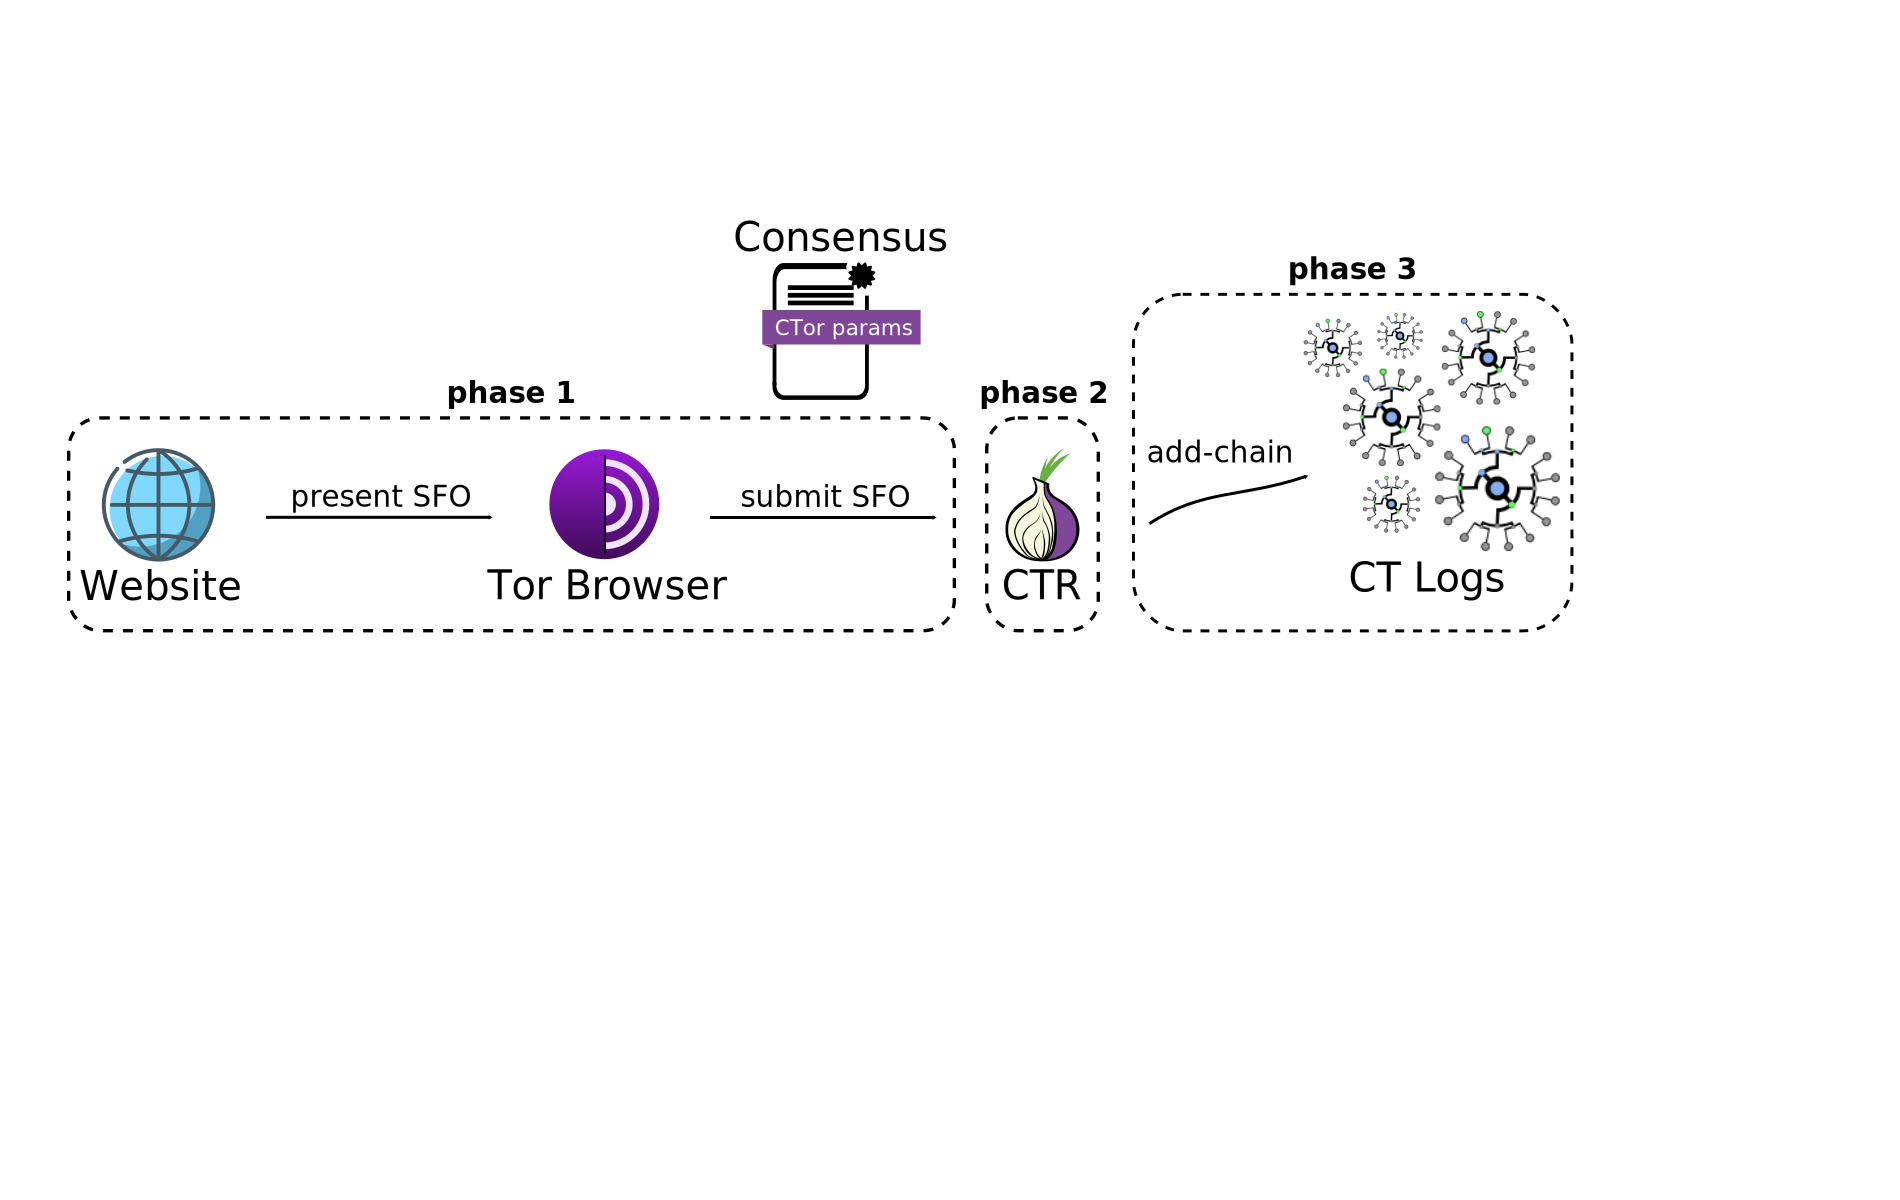
\includegraphics[width=0.85\textwidth]{img/design-ca}
	\caption{%
		The base design of CTor divided into three phases. A website presents an
		SFO to Tor Browser, and Tor Browser in turn with some probability
		submits the SFO to a random CTR (phase 1). A CTR stores the SFO a period
		of time (phase 2). The CTR adds the certificate in the SFO to a random
		independent CT log (phase 3).
	}
	\label{fig:design-ca}
\end{figure*}

\subsection{Tor Consensus} \label{sec:base:consensus}
Our proposal extends Tor's consensus document
so that it entails information regarding
	CTRs,
	recognized CT logs, and
	other necessary parameters that can be tuned.

\subsubsection{CTR Flag} \label{sec:base:consensus:ctr-flag}
The existing \texttt{known-flags} item determines the different flags that a 
given consensus document might contain.  We add another flag named \texttt{CTR},
which indicates that a Tor relay should support CT-auditing as described in
Sections~\ref{sec:base:phase2}--\ref{sec:base:phase3}.  A relay qualifies as a
CTR if it is flagged as \texttt{Stable} and not \texttt{Exit}.  As such, we
suggest using resources that are more abundant when compared to, e.g., exit
bandwidth.  A relay is assigned the \texttt{CTR} flag if a majority of directory
authorities voted for it.

TODO: elaborate 1-2 sentences why this ctr criteria and what it entails (?)

\subsubsection{Recognized CT Log} \label{sec:base:consensus:log}
CTRs only interact with CT logs that are recognized by the Tor consensus.  A log
is recognized if a majority of directory authorities voted for its inclusion by
proposing a \texttt{ct-log-info} entry that contains a log ID, a public key, and
a base URL~\cite{ct,ct/bis}. 
Following from our basic CTR design, there need not be any overlap between the
logs that the Tor consensus recognizes when compared to Tor Browser's CT policy.
There could be overlap, however.  The ideal scenario is that there are many
independent logs that accept certificate chains for most trust anchors.  We
discuss whether this is currently the case or not in Section~\ref{sec:todo}.  In
favor of brevity, details on how the Tor consensus captures whether two logs are
independent and which trust anchors they accept are omitted.

TODO: wrap-up here instead without any forward ref

\subsubsection{Other Parameters} \label{sec:base:consensus:params}
Directory authorities influence the way in which Tor Browser and CTRs behave by
voting on other necessary parameters.  For example, the likelihood that
an SFO is submitted to a CTR is a security parameter that is determined by the
value of \texttt{ct-submit-pr}.  Below, the value of an item is computed as the
median of all votes.
\begin{description}
	\item[ct-submit-pr:] A floating-point in $[0,1]$ that determines Tor
		Browser's submission probability.  For example, $0$ disables submissions
		while $0.10$ means that every 10$^{\mathsf{th}}$ SFO is sent to a
		random CTR on average.
	\item[ct-sfo-max-bytes:] A natural number that determines how many
		wire-bytes a normal SFO should not exceed.  As outlined in
		Section~\ref{sec:base:phase1}, excessively large SFOs are subject
		to stricter verification criteria.
	\item[ct-log-timeout:] A natural number that determines how long a CTR
		waits before concluding that a CT log is unresponsive, e.g., 10~seconds.
		As outlined in Section~\ref{sec:base:phase3}, timeouts trigger implicit
		resubmissions.
	\item[ct-delay-dist:] A distribution that determines how long a CTR should
		wait at minimum before auditing a submitted SFO\@.  As outlined in
		Section~\ref{sec:base:phase2}, random noise is added, e.g., on the order of minutes to an hour.
	\item[ct-backoff-dist:]
		A distribution that determines how long a CTR should wait between two
		auditing instances, e.g., a few minutes on average.  As outlined in
		Section~\ref{sec:base:phase3}, CTRs audit pending SFOs in batches at
		random time intervals to spread out log overhead.
\end{description}

The parameter \texttt{ct-delay-dist} is fulfilling two goals by adding
a randomized delay to the time a CTR should wait before auditing a
submitted SFO\@. For the base design, if a client visits a website and
then an associated SFO is submitted to a CT log shortly thereafter,
this could leak information about client behavior. As an extreme
example, if a known client is unique in visiting a specific collection
of websites together within a short period, seeing associated SFOs for
websites in that collection could indicate to a CT log the behavior of
that client. The randomness in whether a client submits and the
randomness of \texttt{ct-backoff-dist} might help complicate such
leakage. But both of these are primarily for overhead and perfomance,
and the latter is only on the order of minutes. \texttt{ct-delay-dist}
provides a guarantee of behavior obfuscation. 

For the base design, as well as the auditor extension of
Section~\ref{sec:auditor} and log extension of Section~\ref{sec:log},
\texttt{ct-delay-dist} provides some protection against flooding
attacks. Since the available memory of a CTR is known, by flooding
that CTR with enough SFOs before MMD of a mis-issued SCT, the
adversary could flush the desired SFO from the CTR and it would thus
never be audited.  Also for the extensions, if SFOs were audited as
soon as MMD was reached, then an adversary could be more efficient
about knowing when to flood the CTR\@. This could possibly even make
flooding of all CTRs in the network feasible. Even if auditing order
were randomized among all SFOs within an exact interval after MMD (a
timed mix), when to flood a CTR would be predictable. Adding a
randomized delay makes something akin to a stop-and-go mix, except
that the delay time is set by the CTR not the client, which is fine
since this aspect is not to protect client identity but to resist DoS
of SFO audit. Consult the literature~\cite{trickle02} for a description
of mix types.

If the storage strategy against flooding favored preserving SFOs
already at the CTR by dropping inbound SFOs or those farthest from
auditing, the adversary could optimize flooding to just before or
shortly after the mis-issued SFO is sent. If the storage strategy
against flooding favored not blocking incoming SFOs by dropping those
closest to being audited, then the adversary could optimize flooding
to after the mis-issued SFO is sent and as close to MMD as will make
flushing of it likely. To prevent useful optimization of flooding,
when storage capacity at a CTR is exceeded we thus select randomly
from among the pool of received SFOs regardless of time till audit.
And \texttt{ct-delay-dist} similarly complicates any attempted
optimization of when to flood a CTR, thus increasing average cost
of any such DoS attack for the adversary.


\subsection{Phase~1---Tor Browser} \label{sec:base:phase1}
The first phase covers Tor Browser and how an SFO is validated in the TLS
handshake.  We rely on Tor Browser's trust store to check certificate chains, an
assumed SCT-centric CT policy similar to Chrome~\cite{chrome-policy} and
Safari~\cite{safari-policy} to avoid breakage, and \texttt{ct-max-sfo-bytes} as
well as \texttt{ct-submit-pr} to determine whether and how there should be any
follow-up auditing that goes beyond SCT signature verification.  Given an
incoming SFO $s$:

\begin{enumerate}
	\item Raise a certificate error and stop if the certificate chain of $s$
		is not rooted in Tor Browser's trust store.
	\item Raise a certificate transparency error and stop if the SCTs of $s$
		fail Tor Browser's SCT-centric CT policy.
	\item Accept $s$ and conduct the remaining steps in the background if
		$\mathsf{len}(s) \le \texttt{ct-max-sfo-bytes}$, otherwise complete
		all steps and then accept~$s$ as valid.
	\item Flip a biased coin based on \texttt{ct-submit-pr} and stop if the
		outcome indicates no further auditing.
	\item Submit $s$ to a sampled CTR's SFO-endpoint on a pre-built CT-circuit.
		The circuit used for submission is closed immediately after use without
		waiting for any acknowledgment.
\end{enumerate}

In other words, an SFO is accepted as valid if the end-entity certificate is
rooted in a trust anchor \emph{and} it has enough SCTs as dictated by an
SCT-centric CT policy.  The decision and possible submission of an SFO to a
random CTR should never block the TLS handshake under normal circumstances,
whereas \emph{excessively large} SFOs do due to high security risks.  See
Section~\ref{sec:analysis:pr:phase1}, which also motivates why it is paramount
that submission circuits are pre-built and closed as soon as possible.

%
% - close circuit asap to make it harder for an attacker to figure out which
% CTR received a submission (should it have access to a zero-day takeover).
% - clearly a submission circuit cannot be reused across tabs, but not doing
% so within tabs may (i) reduce the chance that the receiving CTR knows exactly
% which website was visited, and (ii) make sense because with small submission
% pr (<=1/10) it should be common to submit at most once per tab anyway.
%

\subsection{Phase 2---Storage} \label{sec:base:phase2}
We suggest that CTRs accept SFO submissions on an HTTP endpoint.\footnote{%
	Tor's HTTP DirServer codebase can be reused as extension point to interact
	with the tor daemon, i.e., add another listener.
} For example, Nordberg~\emph{et~al.} defined an SCT feedback interface that can
be reused if an array-length of one is enforced by the CTR~\cite{nordberg}.
With regards to some CT circuit, process an incoming SFO $s$ as follows:
\begin{enumerate}
	\item\label{enm:storage:close} Close the current circuit to enforce one-time
		usage.
	\item\label{enm:storage:unrecognized} Stop if no CT log in the Tor consensus
		accepts the trust anchor of the underlying certificate chain in $s$.
	\item\label{enm:storage:cached}
		Stop if $s$ is cached or pending to be audited already.
	\item\label{enm:storage:fix-log} Sample an independent CT log $l$ that
		issued no SCT in $s$.  If there are no independent CT logs listed in the
		Tor consensus, sample a dependent CT log instead.
	\item\label{enm:storage:audit-after} Compute an \texttt{audit\_after}
		timestamp $\textrm{t} \gets \mathsf{now()} +
			\mathsf{random}(\texttt{ct-delay-dist})$.
		The former returns the current time and the latter a random delay.
	\item\label{enm:storage:store} Add $(l,t,s)$ to a buffer of pending SFOs.
\end{enumerate}

An SFO that
	(i) cannot be audited with regards to a CT log that the Tor consensus
		recognizes,
	(ii) is already audited as indicated by a \emph{cache}, or
	(iii) is pending to be audited in a \emph{buffer} of pending SFOs,
is discarded.  In contrast, a new SFO is stored in the CTR's buffer
alongside an \texttt{audit\_after} timestamp and a sampled CT log.  The
\texttt{audit\_after} timestamp specifies the earliest point in time that an SFO
will be audited in phase~3, which adds random noise that obfuscate real-time
browsing patterns in the Tor network.  Auditing is also fixed at this stage with
regards to some CT log, notably including resubmissions.  If memory become a
scarce resource, e.g., due to flooding, delete pending SFOs at
random~\cite{nordberg}.

\subsection{Phase 3---Auditing} \label{sec:base:phase3}
Each CTR maintains a single Tor circuit that is used to interact with CT logs
that have \texttt{ct-log-info} items.  At random time intervals, separate
auditing instances are initiated for each of these logs.  Given a known CT log~%
$l$:
\begin{enumerate}
	\item\label{enm:auditing:backoff} Sample a delay $d \gets
		\mathsf{random}(\texttt{ct-backoff-dist})$.
	\item\label{enm:auditing:sleep} Schedule a timer, waiting until $d$
		time units elapsed.
	\item\label{enm:auditing:loop} For each pending buffer entry $(l',s,t)$:
		\begin{enumerate}
			\item\label{enm:auditing:log-check} Continue the loop if $l\ne l'$.
			\item\label{enm:auditing:timestamp-check} Continue the loop if
				$t > \mathsf{now}()$.
			\item\label{enm:auditing:add-chain} Use \texttt{ct-log-timeout} to
				set a timer and add the certificate chain in $s$ to $l$ using
				the public \texttt{add-chain}~\cite{ct} or
				\texttt{submit-entry}~\cite{ct/bis} endpoints.
				\begin{itemize}
					\item\label{enm:auditing:add-chain:success} On valid
						SCT: cache the SFO, then discard it from the buffer of
						pending SFOs.
					\item\label{enm:auditing:add-chain:fail} On any other
						outcome: break the loop.
				\end{itemize}
		\end{enumerate}
	\item\label{enm:auditing:restart} Go back to
		step~\ref{enm:auditing:backoff}.
\end{enumerate}

As shown above we take an unusual approach towards auditing SFOs.  Rather than
following up on an SFO's inclusion status, the underlying certificate chain is
\emph{added} to a random CT log
	(see Section~\ref{sec:base:phase2}, step~\ref{enm:storage:fix-log}).
As such, the end-entity certificate is disclosed to public scrutiny and the
issuing CA will be held accountable if the log in question is honest.  A request
to add the certificate chain is considered successful if a valid SCT is returned
within a timely manner.  On any other outcome, such as invalid SCT signature or
timeout, the SFO remains in the buffer as the loop breaks and the CTR backs-off
in hope that the log becomes available again after wake-up.

Note that the auditing instances of different CT logs are separated.  This
assures that the unavailability of one CT log does not halt auditing of
unrelated buffer entries.

%If there is no independent log listed in the Tor consensus, it is
%still valuable to resubmit to a dependent log:
%	it might be the case that the attacker has access to a log's signing key,
%	but not the log's actual infrastructure.
%In other words, a mis-issued certificate would make it into the public domain
%in such a scenario if we resubmit it rather than discarding it due to lack of
%an independent log.

%%% Local Variables: 
%%% mode: latex 
%%% TeX-master: "../main"
%%% End:          

  \section{Security Analysis} \label{sec:analysis}
TODO: risk, security of base design

  \section{Auditor Extension} \label{sec:auditor}
Until now we have not \emph{verified} whether the certificate chain of an SFO is
publicly logged as promised by the issued SCTs.  As such, it is unlikely that a
misbehaving CT log will be detected.
Our base design can be extended to follow-up
on an SFO's inclusion status rather than adding the underlying certificate chain
to another CT log.  This has the benefit of relaxing our initial trust
assumption, namely that some CT logs are honest, as well as making it possible
to disclose those CT logs that are dishonest.  The downside is added
complexity, which introduces additional threats that must be considered.

\subsection{Design Sketch} \label{sec:auditor:design}
Figure~\ref{fig:auditor} provides an overview of the extended design.  Tor
Browser submits presented SFOs probabilistically to CTRs that are selected at
random, and CTRs store the submitted SFOs before any auditing takes place.
Here, auditing refers to inclusion verification rather than adding certificate
chains.  The moment before auditing, the SFO in question is shared with a CTR
that acts as a \emph{watchdog}.  Unless the auditing CTR receives a timely
inclusion proof and acknowledges it to its watchdog, the (now suspicious) SFO is
reported to a CT auditor.  Phase~1 remains unchanged, some changes are needed
in phase~2, and major changes are required in phase~3 as well as the Tor
consensus.  The extra-info document also includes two new metrics that are
related to flooding.
%Another prerequisite is the existence of CT auditors.

\begin{figure*}
    \centering
    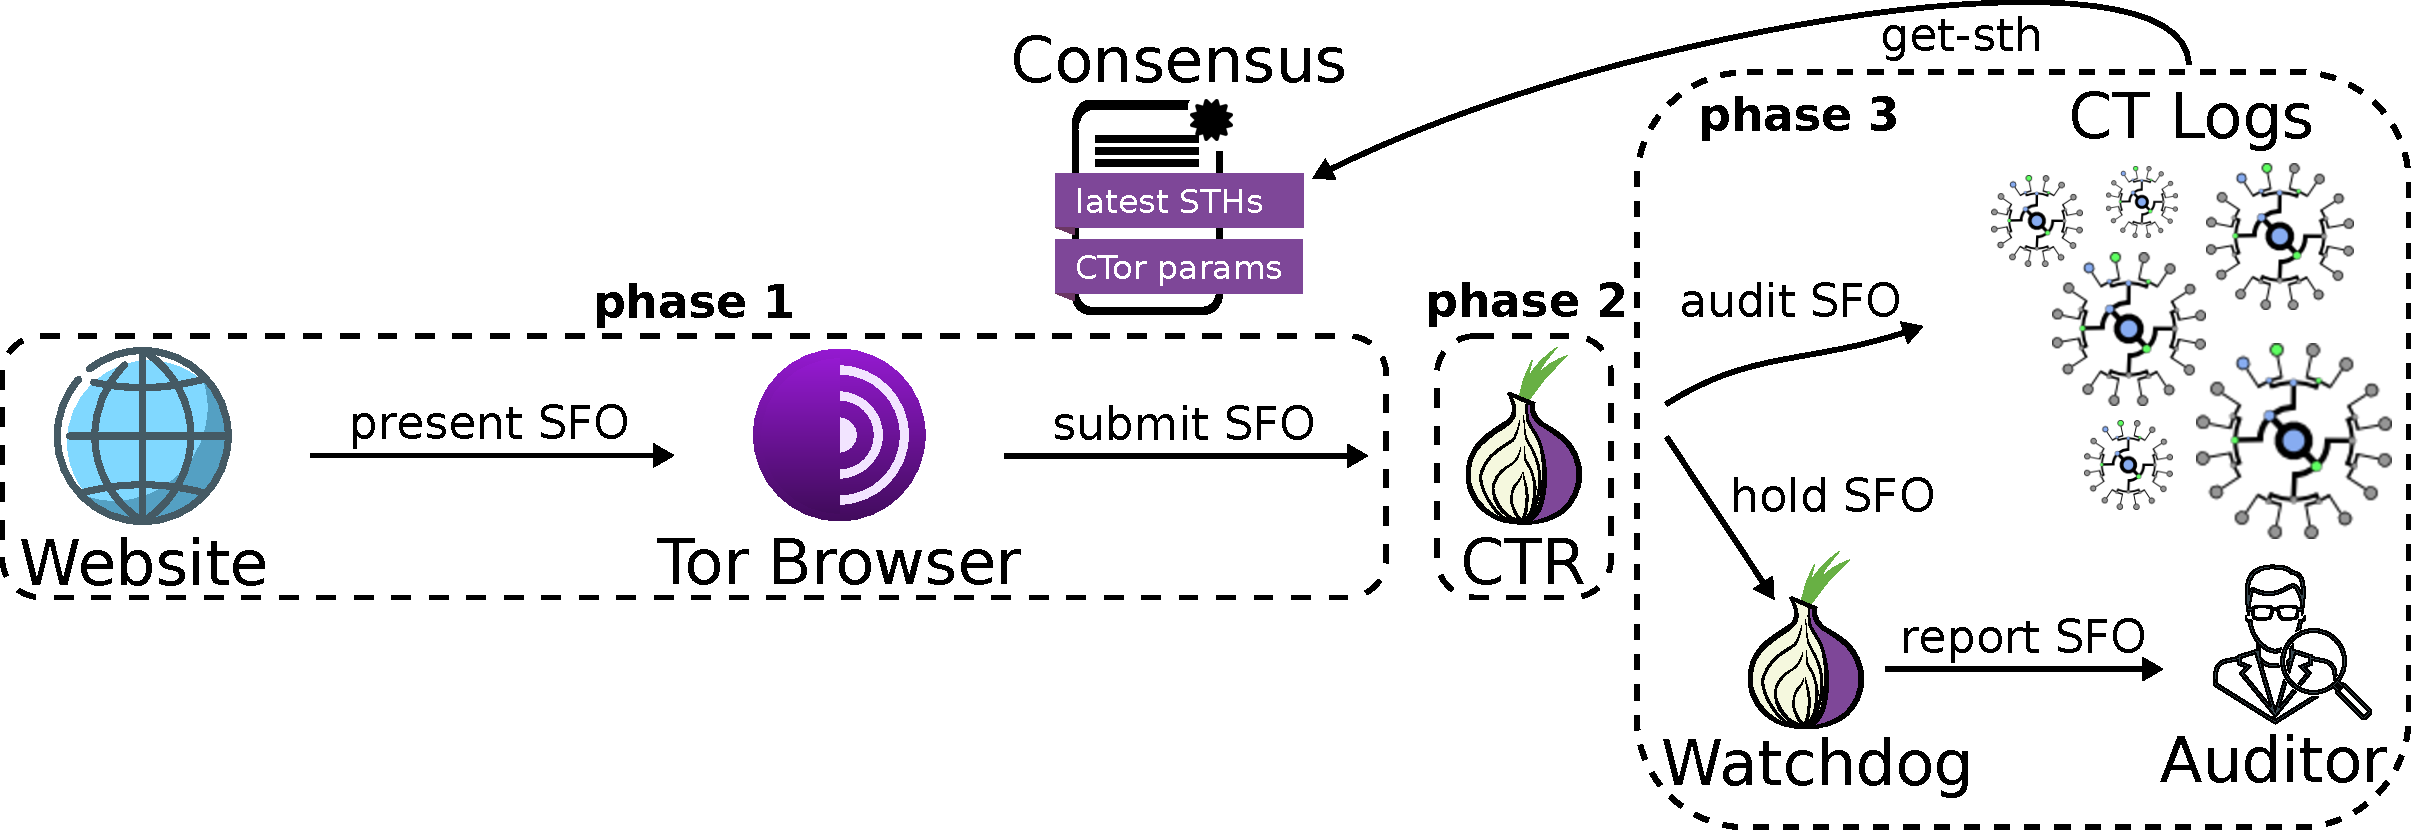
\includegraphics[width=0.85\textwidth]{img/design-auditor}
	\caption{The auditor extension to CTor, where cryptographic evidence of log
	omission can be collected without modification to CT logs. The extension
	changes the consensus to include the latest STHs from CT logs and makes
	phase 3 significantly more complex. CTRs in phase 3 now challenge logs to
	prove inclusion of certificates from SFOs, using other CTRs as
	``watchdogs'', ensuring that SFOs that are not provably correct are reported
	to trusted auditors.}
	\label{fig:auditor}
\end{figure*}

\subsubsection{Tor Consensus} \label{sec:auditor:design:consensus}
Tor's consensus should capture a fixed view of the CT landscape by publishing
STHs from all recognized logs.  A CT log is recognized if a majority of directory
authorities proposed a \texttt{ct-log-info} item, which contains a log's ID,
public key, base URL, MMD, and most recent STH.  Note that each directory
authority proposes its own STH, and agrees to use the most recent STH as
determined by timestamp.  Since CTRs verify inclusion statuses of SCTs
that Tor Browser accepts, the CT logs recognized by Tor Browser must be in
Tor's consensus.

Tor's directory authorities also majority-vote on \texttt{ct-auditor} items,
which pin base URLs and public keys of CT auditors that watchdogs contact in
case that any log misbehavior is suspected.  A watchdog triggers if the time
specified by \texttt{ct-watchdog-timeout} elapses without receiving any
acknowledgment.  The following auditor submission is governed by a
\texttt{ct-auditor-timeout}, which, if triggered, results in a resubmission
later on.

\subsubsection{Phase~2---Storage} \label{sec:auditor:design:phase2}
Other than updating the criteria of what it means that an SFO can be audited
in phase~3, the computation of $l$ and $t$ changes for a buffer's entry.  With
regards to some CT circuit, process an incoming SFO $s$ as follows:
\begin{enumerate}
	\item\label{enm:ext:storage:close} Close the current circuit to enforce
		one-time usage.
	\item\label{enm:ext:storage:unrecognized} Discard unrecognized SCTs in $s$
		whose logs have no corresponding \texttt{ct-log-info} items listed in
		the Tor consensus.  Stop if there are no remaining SCTs in~$s$.
	\item\label{enm:ext:storage:cached}
		Stop if $s$ is cached or pending to be audited already.
	\item\label{enm:ext:storage:fix-log} Sample a CT log $l$ that issued a
		remaining SCT in~$s$.
	\item\label{enm:storage:audit-after} Compute an \texttt{audit\_after}
		time~$t$, see Figure~\ref{fig:audit-after}.
	\item\label{enm:storage:store} Add $(l,t,s)$ to a buffer of pending SFOs.
\end{enumerate}

Recall from Section~\ref{sec:background:ct} that an inclusion proof is fetched
with regards to an STH.  As such, we discard SCTs that cannot be verified due to
lack of \texttt{ct-log-info} items in the Tor consensus.  The sampled CT log $l$
now refers to an entity that issued an SCT in the submitted SFO, and it will be
challenged to prove inclusion in phase~3 sometime after the
\texttt{audit\_after} timestamp $t$ elapsed.  Figure~\ref{fig:audit-after} shows
that $t$ takes the log's MMD into account.  This is one of two parts that
prevent \emph{early signals} to the issuing CT logs that an SFO is being
audited.  For example, if an SFO is audited before the MMD elapsed, the issuing
CT log could simply merge the underlying certificate chain to avoid an MMD
violation.  This would not yield any improvement with regards to the base
design.

\begin{figure}
	\centering
	\pseudocode[linenumbering, syntaxhighlight=auto]{%
		\textrm{t} \gets \mathsf{now}() +
			\mathsf{MMD} +
			\mathsf{random}(\texttt{ct-delay-dist}) \\
		\pcif \textrm{SCT.timestamp} + \textrm{MMD} <
				\mathsf{now}():\\
			\pcind\textrm{t} \gets \mathsf{now}() +
				\mathsf{random}(\texttt{ct-delay-dist})
	}
	\caption{%
		Algorithm that computes an \texttt{audit\_after} timestamp $t$.
	}
	\label{fig:audit-after}
\end{figure}

\subsubsection{Phase~3---Auditing} \label{sec:auditor:design:phase3}
In addition to maintaining a single Tor circuit that is used to interact with
CT logs that have \texttt{ct-log-items}, a distinct Tor circuit is maintained
and rotated that ends at a random watchdog CTR.  Given a known CT log
$l$:
\begin{enumerate}
	\item\label{enm:ext:auditing:backoff} Sample a delay $d \gets
		\mathsf{random}(\texttt{ct-backoff-dist})$.
	\item\label{enm:ext:auditing:sleep} Schedule a timer, waiting until $d$
		time units elapsed.
	\item\label{enm:auditing:loop} For each pending buffer entry $(l',s,t)$:
		\begin{enumerate}
			\item\label{enm:ext:auditing:log-check}
				Continue the loop if $l\ne l'$.
			\item\label{enm:ext:auditing:timestamp-check} Continue the loop if
				$t > \mathsf{now}()$.
			\item\label{enm:ext:auditing:sth-check} Continue the loop if $t >
				\textrm{STH}.\mathsf{timestamp}$.
			\item\label{enm:ext:auditing:watchdog} Share $s$ with the current
				watchdog.
			\item\label{enm:ext:auditing:challenge} Use \texttt{ct-log-timeout}
				and $\textrm{STH}.\mathsf{treesize}$ to set a timer and
				challenge the log to prove inclusion.
				\begin{itemize}
					\item\label{enm:ext:auditing:challenge:success} On valid
						proof: send an acknowledgment to the watchdog, then
						cache $s$ and discard it.
					\item\label{enm:ext:auditing:challenge:fail} On any other
						outcome: discard $s$ and break.
				\end{itemize}
		\end{enumerate}
	\item\label{enm:ext:auditing:restart} Go back to
		step~\ref{enm:ext:auditing:backoff}.
\end{enumerate}

An SFO is not audited for inclusion until the log's MMD elapsed \emph{and} there
is an STH in the Tor consensus that captures it.  As such, a CT log that intends
to omit a certificate chain despite promising to merge it within its MMD will
not get an early signal that a CTR will audit it.
Before auditing, the SFO in question is shared with a watchdog that takes on
the responsibility of reporting suspicious SFOs to the pinned CT auditors.
An SFO is considered suspicious if it is not acknowledged by the log-challenging
CTR as verified within the time specified by \texttt{ct-watchdog-timeout}.  As
argued in Section~\ref{sec:auditor:analysis:phase3}, it is motivated to use a
watchdog:
	the attacker learns which CTR holds the problematic SFO at the time of
		auditing, and
	during the \texttt{ct-log-timeout} actions could then be taken to ensure
		that the SFO does not reach a CT auditor.
A watchdog that receives a suspicious SFO reports it to a random CT auditor,
and resubmits it later on if the \texttt{ct-auditor-timeout} happens to trigger.

\subsubsection{Extra-Info Document} \label{sec:auditor:extra-info}
Following from the \texttt{audit\_after} timestamp algorithm in
Figure~\ref{fig:audit-after}, an SFO may be stored throughout an entire MMD.
This results in a relatively large time window during which the attacker can
attempt to flood all CTRs in hope that they delete the omitted SFO at random
before it is audited.  We discuss the threat of flooding further in
Section~\ref{sec:auditor:analysis:phase2}, noting that it can be detected if
CTRs publish two new metrics in the extra-info document:
	\texttt{ct-receive-bytes} and
	\texttt{ct-delete-bytes}.
These metrics indicate how many SFO bytes were received and deleted throughout
different time intervals, which is similar to other extra-info metrics such
as \texttt{read-history}.

\subsubsection{CT Auditor} \label{sec:auditor:auditor}
An announced auditor is expected to accept SFOs at a dedicated endpoint,
endeavoring to validate the inclusion status of each SCT with regards to the
first STH in the Tor consensus that elapsed the log's MMD.  If a log appears to
function correctly except for some evidence that cannot be
resolved despite multiple attempts that span a given time period, it is
paramount that the auditor software alerts its operator who can investigate
the issue further before submitting a full report to the CT-policy mailing list.
Cases of misbehavior, in detail:
\begin{itemize}
	\item If the log fails to provide a valid inclusion proof for an SCT with
		regards to the first applicable STH in the Tor consensus
		(certificate omission).
	\item If the log fails to provide a valid consistency proof between two
		STHs in the Tor consensus
		(split-view).
	\item If a published STH is future-dated or backdated more than an MMD
		(general log misbehavior).
	\item If a log ignores some CTRs (uptime misbehavior).
\end{itemize}

An unresponsive log can be suspected by observing the watchdog report frequency,
and possibly confirmed by querying the log in question from different vantage
points.  Among other extra-info metrics that go beyond received and deleted
SFO-bytes that the announced CT auditors should check, it could be valuable to
publish the extent to which CTR-to-log interactions fail.

%While not within our threat model, we do encourage the announced auditors to
%verify that STHs in the Tor consensus are consistent with external views of the
%CT landscape.  For example, operate an STH pollination~\cite{nordberg} endpoint
%and fetch STHs actively from many diverse vantage points using Tor, VPN
%services, DoH resolvers, and RIPE Atlas (to mention a few low-cost options).
%This goes back to the point of general ecosystem value.
% => this is now a "forward point"

%TODO: all flushing and tagging details here
\subsection{Security Analysis} \label{sec:auditor:analysis}
Idea: go through what is \emph{different} with regards to the base analysis.

Make sure it is clear why we do delete at random before analysis starts

\subsubsection{Phase~2---Storage} \label{sec:auditor:analysis:phase2}
The main difference with regards to the base design is that an SFO can be
stored much longer.  The attacker can maximize the \texttt{audit\_after}
timestamp by using a newly issued SFO, resulting in a storage phase of \emph{at
least} an MMD.  This time can be extended further by delaying issuance of an
STH that would capture the omission:
	a log must produce an STH every MMD~\cite{ct,ct/bis}.
This means that the maximized storage time is in the order of two MMDs; not
considering that it also takes time for an STH to be propagated into the Tor
consensus.  Most logs use an MMD of 24~hours, resulting in an attack window that
ranges from one to two days.  A risk-averse attacker should prefer to use the
lower bound:
	suddenly not issuing any new STH is visible, attracting attention.

Following from Tor's threat model, the mis-issued SFO must be stored in
volatile memory and not to disk.  Two risks emerge as a result of the increased
storage time:
	the CTR in question might be restarted by the operator,
	and the attacker might \emph{flood} it by submitting many SFOs with the
		intent to \emph{flush} a target entry from the buffer~\cite{nordberg}.
A risk-averse attacker cannot rely on the former, but the latter is applicable
if all CTRs can be targeted without making Tor unavailable.
Appendix~\ref{app:flush} shows that the number of SFO submissions~$k$
that the attacker needs to successfully flush a buffer of $n>1$ entries with
some probability~$p<1$ is given by Equation~\ref{eq:flush}.
\begin{equation} \label{eq:flush}
	k = \frac{\log(1-p)}{\log(1 - \frac{1}{n})}
\end{equation}

It is recommended that a non-exit relay should have at least 512~MB of memory.
If the available bandwidth exceeds 40~Mbps, it should have at least
1~GB~\cite{relay-config}.  Given that these recommendations are lower bounds,
suppose the average memory available to store SFOs is 1~GiB.  Further, our
dataset in Section~\ref{sec:performance} shows that the average SFO is in the
order of 6~KiB.  This means that the buffer capacity is $n \gets 174763$ SFOs.
Plugging it into Equation~\ref{eq:flush} for $p \gets \frac{9}{10}$, the
attacker's flood must involve $k \gets 402406$ submissions.  In other words,
2.3~GiB must be transmitted to flush a single CTR,\footnote{%
	As a corner case and implementation detail, it is important that Tor Browser
	and CTRs \emph{reject} SFOs that are bogus in terms of size:
		it is a trivial DoS vector to load data indefinitely.
	Analysis based on, e.g., 1~MiB SFOs also requires 2.3~GiB of data to flush.
} which takes $7.9$--$39.3$~minutes if its bandwidth is between 8 and 40~Mbps.
Thus, it is impractical to flush all CTRs within minutes.

Metrics reported by the Tor project show that there are over 4000 relays that
match our CTR criteria~\cite{relay-by-flag}.  As such, a network-wide flush
involves the transmission of at least 8.99~TiB.  It might sound daunting at
first, but distributed over a day it only requires 0.91~Gbps.  While we cannot
avoid early signals to the logs \emph{and} at the same time prevent flushing
without writing anything to disk, it is detectable based on the extra-info
document.  On the flip-side, \emph{not observing any flushing} adds a large
degree of confidence that there are no mis-issued SFOs.

\subsubsection{Phase~3---Auditing} \label{sec:auditor:analysis:phase3}
%Now we are talking to the attacker.  Attacker learns that a mis-issued SFO
%is being audited.  Auditing happens over a shared Tor circuit, and despite the
%anonymity that it provides, the attacker can overcome it by tagging.  Briefly
%explain tagging.
%
%If the CTR submitted to a CT auditor, it would leave a ~seconds window where
%the attacker could simply DoS an identifiable CTR.  Therefore, we delegated
%reporting to a random watchdog \emph{before} doing the inclusion query.
%The attacker does not learn the watchdog identity unless we sample the
%attacker's CTR.  We do not consider the threat of fully taking over the Tor
%relay within seconds to identify the watchdog; too strong for Tor's threat
%model.

% MISC notes
% - Network-wide flush, detectable but hard to attribute
% - Requires new reliable auditor software
% - Bit more bandwidth due to watchdog.  The overhead, when compared to log a
% log extension, is sending an SCT hash and receiving a proof (2-3KiB).
% - A rational attacker is the issuer of all SCTs in the omitted SFO, so it is
% sufficient to verify inclusion with regards to one SCT and then leave it to
% the auditors to bust all involved CT logs.


  \section{Log Extension} \label{sec:log}
If we allow small, but significant, changes to the CT landscape, it is possible
to avoid inclusion verification and the involved complexities as described in
Section~\ref{sec:auditor}.  The idea is based on returning back to the premise
of some, but not all, CT logs being honest.  However, the goal is not only
\emph{resilience towards} but also \emph{detection of} CT logs that misbehaved.
The extended design idea is nearly identical to the base design, as was shown in
Figure~\ref{fig:design-ca}.  Tor Browser submits presented SFOs
probabilistically to CTRs that are selected at random in phase 1, and CTRs store
the submitted SFOs in phase 2 before any \emph{auditing} takes place in phase 3.
Here, auditing refers to adding an SFO to an independent CT log; not just the
underlying certificate chain.  This is the main difference in the log extension.
By also adding the issued SCTs, the associated CT logs can be held accountable
for possible omissions.

The prerequisite for such an extension to work is that CT logs support an
additional API endpoint:
	\texttt{add-sfo}.
First we describe how this endpoint could be operated so that \emph{the only
change} with regards to the base design in Section~\ref{sec:base} is that
certificate chains and SCTs are added.  Next, we explain how some of the log's
complexity could be moved into the Tor landscape at the cost of bringing back
the threat of flooding as discussed in
Section~\ref{sec:auditor:analysis:phase2}.

\textbf{Approach~1.}
Recall from Section~\ref{sec:auditor:design:phase2} that there must not be any
early signals that allow misbehaving CT logs to reactively merge certificate
chains before any MMD promise is violated.  To ensure that this is the case, the
\texttt{add-sfo} endpoint could entail a promise that the added SFO will not be
merged until all MMDs elapsed.\footnote{%
	Two options: just base on MMD and wait ``long enough'', or wait until the
	log created an actual STH.  TODO: refactor me.
} For example, the SCT that is returned by the \texttt{add-sfo} endpoint could
have a future-dated timestamp without violating any policy aspect of
CT/bis~\cite{ct/bis}.  Note that the appeal of letting CT logs handle
\emph{delayed merges} is that no attacker within Tor's threat model have high
certainty of succeeding with a network-wide flush.

\textbf{Approach~2.}  The other option is to suggest minimal changes to the CT
landscape by operating the \texttt{add-sfo} endpoint without any other
expectation than that it must allow SCTs in addition to a certificate chain.
To avoid early signals, CTRs should adopt the procedures in
Sections~\ref{sec:auditor:design:phase2}--\ref{sec:auditor:design:phase3}
or something similar.  For example, \texttt{audit\_after} timestamps
could be computed conservatively as in Figure~\ref{fig:audit-after-cons}
to remove the dependency of STHs in the Tor consensus.  There is a threat of
network-wide flushes regardless, and the extra-info document should therefore be
extended as in Section~\ref{sec:auditor:extra-info}.

%
% TODO:
% Think we need either 2*MMD as the log must produce an STH every MMD.  Or,
% have STHs in the consensus after all which would be more robust.
%
\begin{figure}
	\centering
	TODO: discuss and docdoc.
	\caption{%
		Algorithm that computes a conservative \texttt{audit\_after} timestamp
		$t$.
	}
	\label{fig:audit-after-cons}
\end{figure}

  \section{Discussion} \label{sec:discussion}

\subsection{Privacy}
At least mention privacy leaks to auditor. For example, related to CT logs uptime.
  %Paul: mixing?
% cite does-ct-break-the-web somewhere as motivation of TB's SCT CT policy
\section{Related Work} \label{sec:related}
Google's Chrome and Apple's Safari enforce CT by mandating that every TLS
certificate must be accompanied by two independent
SCTs~\cite{chrome-policy,safari-policy}.  We proposed that Tor Browser should
follow suit, but, unlike any other web browser that enforces CT, CTor provides
\emph{concrete next steps} that relax the centralized trust which is otherwise
and evidently misplaced in CT logs~\cite{%
	izenpe-disqualified,%
	venafi-disqualified,%
	gdca1-omission,%
	digicert-log-compromised%
}.

%%%
% Privacy preserving inclusion proofs
%%%
Laurie proposed that inclusion proofs could be fetched over DNS to avoid
additional privacy leaks, i.e., a user's browsing patterns are already exposed
to the DNS resolver but not the logs in the CT landscape~\cite{ct-over-dns}.
CT/bis provides the option of serving stapled inclusion proofs as part of the
TLS handshake in an extension, an OCSP response, or the certificate
itself~\cite{ct/bis}.
Lueks and Goldberg proposed that a separate database of inclusion proofs could
be maintained that supports information-theoretic PIR~\cite{lueks-and-goldberg}.
Kales~\emph{et~al.} improved scalability by reducing the size of each entry
in the PIR database at the cost of transforming logs into multi-tier Merkle
trees, and additionally, showed how the upper tier could be expressed as
a two-server computational PIR database to ensure that any inclusion proof can
be computed privately on-the-fly~\cite{kales}.
Nordberg~\emph{et~al.} avoid inclusion proof fetching by hanging on to presented
SFOs, handing them back to the same origin at a later time~\cite{nordberg}.
In contrast, CTor protects the user's privacy without any persited browser state
by submitting SFOs on independent Tor circuits to CTRs, which in turn add random
noise before there is any log interaction to speak of.  The use of CTRs
enable caching similar to CT-over-DNS, but it does not put the logs in the dark
like PIR could.

%%%
% The same consistent view
%%%
Inclusion proofs are only meaningful if everyone observes the same consistent
STHs.
One option is to configure client software with a list of entities that they
should gossip with, e.g., CT monitors~\cite{chase}, or,
browser vendors could push a verified view~\cite{sth-push}.
Such trusted auditor relationships may work for some but not
others~\cite{nordberg}.
Chuat~\emph{et~al.} proposed that HTTPS clients and HTTPS servers could pool
STHs and consistency proofs which are gossiped on website visits~\cite{chuat}.
Nordberg~\emph{et~al.} suggested a similar variant, reducing the risk of user
tracking by pooling fewer and recent STHs~\cite{nordberg}.
Dahlberg~\emph{et~al.} noted that such privacy-insensitive STHs need not be
encrypted, which could enable network operators to use programmable data planes
to provide gossip as-a-service~\cite{dahlberg}.
Syta~\emph{et~al.} proposed an alternative to reactive gossip mechanisms by
showing how an STH can be cosigned efficiently by many independent
witnesses~\cite{syta}.
A scaled-down version of witness cosigning could be instantiated by
cross-logging STHs in other CT logs~\cite{minimal-gossip},
or, in other append-only ledgers~\cite{catena}.
CTor's extended design in Section~\ref{sec:auditor} ensures that anyone
connected to the Tor network is on the same view by making STHs public in the
Tor consensus.  In contrast, the base design is not about catching log
misbehavior, and the extended design in Section~\ref{sec:log} exposes logs
that misbehave \emph{without} fetching inclusion proofs.

Nordberg proposed that Tor clients could enforce public logging of consensus
documents and votes~\cite{consensus-transparency}.  Such an initiative is
mostly orthogonal to CTor, as it strenghtens the assumption of a secure Tor
consensus by enabling detection of compromised signing keys rather than
mis-issued TLS certificates.  Winter~\emph{et~al.} proposed that Tor Browser
could check self-signed TLS certificates for extact matches on independent Tor
circuits.  Alicherry~\emph{et~al.} proposed that any web browser could
double-check TLS certificates on first encounter using alternative paths and
Tor, again, looking for certificate mismatches and generating warnings of
possible man-in-the-middle attacks~\cite{doublecheck}.  The submission phase in
CTor is similar to such double-checking, expect that there is no normal-case TLS
handshake blocking, browser warnings, or strict assumptions regarding the
attacker's location.

  \section{Conclusion} \label{sec:conclusion}
CTor consists of a base design and two possible extensions with the goal of
adding incremental and privacy-preserving support for Certificate Transparency
to Tor. The use of relays in the Tor network distributes caching of observed
SFOs and delays interactions with CT logs, central to both overall security and
preserving privacy of Tor users. Our analysis also shows that these relays are
the weakest link: the most promising chance of avoiding exposure of compromising
SFOs appears to be to attempt to perform network-wide DoS on relays, or attack
CT logs directly. 

Mitigation of network-wide attacks take us outside of Tor's---and therefore also
our---threat model. That said, we cannot ignore such attacks given the strong
attacker we consider (to some degree in control of both a trusted CA and CT
logs). Several parameters of our design enables Tor to \emph{adapt} to observed
interference with CTor, such as a network-wide DoS of relays, reported targeted
attacks of CT logs, or relays reporting suspected flooding through the
\texttt{ct-delete-bytes}  extra-info. When it comes to TB, the submission
probability (\texttt{ct-submit-pr}) and SFO size threshold
(\texttt{ct-max-sfo-bytes}) could be set such as to force all SFOs to be sent to
a CTR before accepting any new HTTPS application-layer data. During the storage
phase, the consensus specifies each CT log's MMD and the delay distribution
(\texttt{ct-delay-dist}), which can be set to either minimize or maximize the
delay between TB user and CT log interaction. Similarly, trusted auditors
(auditor extension) and log operator relationships (base design and log
extension) are also defined in the consensus and can be tweaked.

Deploying CTor, in particular with the log extension that requires trusted
auditors, would be a significant operational burden. Overall Tor network health
would have to include considerations of tweaking CTor parameters to adapt to
strong attackers. However, the potential gains are significant. Tor users would
benefit from the significant security improvement provided by CT logs. Perhaps
more significantly, Tor would be a system for maintaining a
probabilistically-audited cryptographically-verifiable view of the entire CT log
ecosystem available from Tor’s consensus. This would benefit the wider web and
Internet, since the view from Tor's consensus could serve as a base of trust,
relaxing the necessary trust that currently has to be placed on CT log
operators. As a starting point, our base design turns Tor Browser into a helpful
participant in addressing the weakest-link issue of the CA ecosystem, in line
with the goals of CT.


  \bibliographystyle{abbrv}
  \bibliography{src/ref}

  %\appendix
  %\section{Extra}
\end{document}
